\section{Обзор предметной области}
\label{sec:domain}

В данном разделе будет произведён обзор предметной области задачи, решаемой в рамках дипломного проекта; рассмотрены алгоритмы для работы с текстовыми данными и развитие технологмй в данном направлении. Также будут рассмотрены подходы к решению задачи языкового моделирования.

\subsection{Natural Language Processing}
\label{sub:domain:nlp}

Natural Language Processing (NLP) --- область машинного обучения, связанная с предоставлением компьютерам возможности понимать текст и произносимые слова почти так же, как люди.

NLP сочетает в себе вычислительную лингвистику — моделирование человеческого языка на основе правил — со статистическими моделями, машинным обучением и моделями глубокого обучения. Вместе эти технологии позволяют компьютерам обрабатывать человеческий язык в виде текстовых или голосовых данных и «понимать» его полное значение, включая намерения и чувства говорящего или пишущего.

NLP управляет компьютерными программами, которые переводят текст с одного языка на другой, реагируют на голосовые команды и быстро резюмируют большие объемы текста — даже в режиме реального времени. В повседневной жизни многие взаимодействовали с NLP в виде голосовых систем GPS, цифровых помощников, программного обеспечения для преобразования речи в текст, чат-ботов для обслуживания клиентов и других сервисов. Но NLP также играет все более важную роль в корпоративных решениях, помогающих упростить бизнес-операции, повысить производительность сотрудников и упростить критически важные бизнес-процессы.

Человеческий язык полон двусмысленностей, которые невероятно затрудняют написание программного обеспечения, точно определяющего предполагаемое значение текстовых или голосовых данных. Омонимы, омофоны, сарказм, идиомы, метафоры, исключения из грамматики и использования, вариации в структуре предложений — это лишь некоторые из особенностей человеческого языка, на изучение которых у людей уходят годы, однако приложения должны изначально уметь это распознавать, чтобы приносить какую-либо пользу.

Некоторые задачи NLP требует обработки одновременно и текстовых, и гоосовых данных. К ним относятся: 

\begin{itemize}
	\item Распознавание речи, что представляет собой задачу надежного преобразования голосовых данных в текстовые. Распознавание речи требуется для любого приложения, которое следует голосовым командам или отвечает на голосовые запросы. Что делает распознавание речи особенно сложным, так это то, как люди говорят: быстро, невнятно, с разным ударением и интонацией, с разным акцентом и часто с использованием неправильной грамматики.
	
	\item Тегирование частей речи, также называемое грамматическим тегированием, представляет собой процесс распознавания части речи определенного слова или фрагмента текста на основе его использования и контекста.
	
	\item Устранение неоднозначности смысла слова --- это выбор значения слова с несколькими значениями посредством процесса семантического анализа, который определяет слово, которое имеет наибольший смысл в данном контексте.
	
	\item Распознавание именованных сущностей, или Named Entity Recognition (NER), идентифицирует слова или фразы как полезные сущности. NER позволяет по слову и его контексту понять, это имя человека, город или какой-либо иной объект.
	
	\item Анализ эмоциональной окраски пытается извлечь из текста субъективные качества — отношение, эмоции, сарказм, замешательство, подозрительность.
	
	\item Генерация естественного языка ---  это задача перевода структурированной информации на человеческий язык.~\cite{ibm_nlp}
\end{itemize}

\subsection{Задача языкового моделирования}
\label{sub:domain:language_modeling}

Языковое моделирование (Language Modeling или LM) — это использование различных методов для определения вероятности появления данной последовательности слов в предложении. Языковые модели анализируют массивы текстовых данных, чтобы обеспечить основу для своих предсказаний. Они используются для решения задач, связанных с обработкой естественного языка и при генерации текста. К таким задачам среди прочих относятся машинный перевод и ответы на вопросы.

Основная цель в языковом моделировании --- оценить вероятности текстовых фрагментов. Мы хотим, чтобы эти вероятности отражали знание языка. В частности, мы хотим, чтобы предложения, которые «с большей вероятностью» появятся в языке, имели большую вероятность в соответствии с нашей языковой моделью. Вероятности последовательностей оцениваются по формуле условной вероятности:
\begin{equation}
	P(y_1, y_2,...,y_n) = P(y_1) \cdot P(y_2|y_1) \cdot P(y_3|y_1, y_2) \cdot ... \cdot P(y_n|y_1,...,y_{n-1}) = \prod_{t=1}^n{P(y_t|y_{<t})}
\end{equation}
Благодаря данной формуле мы можем преобразовать вероятность последовательности в произведение условных вероятностей отдельных слов или токенов.~\cite{lena-voita-lm}

Языковые модели определяют вероятность слова, анализируя текстовые данные. Они интерпретируют эти данные, пропуская их через алгоритм для получения контекстной информации. Затем модель применяет эту информацию в языковых задачах, чтобы точно прогнозировать или создавать новые предложения. Модель по существу изучает особенности и характеристики языка и использует эти знания для понимания новых фраз.

Методы языкового моделирования:
\begin{itemize}
	\item N-грамм. N-граммы — это относительно простой подход к языковым моделям. Они создают распределение вероятностей для последовательност длины $n$. $n$ может быть любым числом и определяет размер последовательности слов, которым присваивается вероятность. По сути, $n$ можно рассматривать как объем контекста, который модель должна учитывать. Некоторые типы n-грамм — это униграммы, биграммы, триграммы и так далее.
	
	\item Униграмма. Униграмма — простейший тип языковой модели. В вычислениях не рассматривается какой-либо контекст. Модель оценивает каждое слово или термин независимо. Модели Unigram обычно решают задачи обработки языка, такие как поиск информации. Униграмма является основой более конкретного варианта модели, называемой моделью вероятности запроса, которая использует поиск информации для изучения пула документов и поиска наиболее релевантного для конкретного запроса.
	
	\item Двунаправленный. В отличие от моделей n-грамм, которые анализируют текст в одном направлении (назад), двунаправленные модели анализируют текст в обоих направлениях, назад и вперед. Эти модели могут предсказать любое слово в предложении или теле текста. Двунаправленное изучение текста повышает точность результатов. Этот тип часто используется в приложениях для машинного обучения и генерации речи. Например, Google использует двунаправленную модель для обработки поисковых запросов. Однако такие модели не подходят для генерации текстовых последовательностей.
	
	\item Экспоненциальный. Этот тип, также известный как модели максимальной энтропии, сложнее, чем n-граммы. Проще говоря, модель оценивает текст с помощью уравнения, которое объединяет функции признаков и n-граммы. По сути, этот тип определяет характеристики и параметры желаемых результатов и, в отличие от n-грамм, оставляет параметры анализа более неоднозначными — например, он не указывает размеры отдельных граммов. Модель основана на принципе энтропии, согласно которому распределение вероятностей с наибольшей энтропией является наилучшим выбором. Другими словами, модель с наибольшим хаосом и наименьшим количеством предположений является наиболее точной. Экспоненциальные модели основаны на максимизации кросс-энтропии, которая сводит к минимуму количество статистических предположений.
	
	\item Нейросетевой. Этот тип модели представляет слова как нелинейную комбинацию весов в нейронной сети. Веса слов называются эмбеддингами (embedding). Этот тип становится особенно полезным по мере того, как наборы данных становятся все больше, потому что большие наборы данных часто включают больше уникальных слов. Наличие большого количества уникальных или редко используемых слов может вызвать проблемы для линейной модели, такой как n-грамма. Это связано с тем, что количество возможных последовательностей слов увеличивается, а шаблоны, определяющие результаты, становятся слабее. Взвешивая слова нелинейным, распределенным способом, эта модель может «научиться» аппроксимировать слова и, следовательно, не будет введена в заблуждение какими-либо неизвестными значениями. Его «понимание» данного слова не так сильно привязано к непосредственно окружающим словам, как в моделях n-грамм.
\end{itemize}

Языковое моделирование имеет решающее значение при решении современных задач анализа текстовых данных. Именно благодаря им машины могут понимать качественную информацию. Каждый тип языковой модели тем или иным образом превращает качественную информацию в количественную. Это позволяет людям в ограниченной степени общаться с машинами так же, как они общаются друг с другом. 

Языковые модели применяются в различных отраслях, включая технологии, финансы, здравоохранение, транспорт, юриспруденцию и другие. Кроме того большинство людей, каким-то образом взаимодействуют с языковой моделью в на ежедневной основе, будь то поиск Google, функция автозаполнения текста или взаимодействие с голосовым помощником.~\cite{language_modeling_abstract}

\subsection{История языкового моделирования}

Языковое моделирование имеет довольно насыщенную историю. Впервые n-грамные модели упоминались в статье~\cite{shannon-math-theory-of-communication} еще в 1948 году, где описывалось применение марковских цепей для создания статистической модели для последовательностей символов в сообщениях на английском языке. В 1970 году финским студентом Seppo Linnainmaa был предложен в современном виде алгоритм backpropagation~\cite{backprop_first_mention}, который в дальнейшем ляжет в основу 99.9\% всех нейросетей.

В 1980 годах основные исследования все еще были сосредоточены на статистических методах, однако вместе с этим появилось несколько методов нейросетевого моделирования, которые найдут применение в дальнейшем. В 1982 появилась идея рекуррентных нейросетей, описанных в статье J. Hopfield \cite{hopfield_rnn}. Данные сети не имеют ничего общего с современными рекуррентными нейросетями, так как не способны обрабатывать последовательности данных, однако заложили основу для дальнейших исследований. В 1986 году более глубоко рассматривалось применение backpropagation (или метод обратного распространения ошибки) в рекуррентных сетях для генерации последовательностей~\cite{rumelhart_backprop}. Также возникла идея представления различных символом или слов в виде векторов. Однако полноценной нейросетевой моделью для языкового моделирования это считать нельзя, так как эксперименты проводились на искусственных данных и с малым количеством различных символов.

В 1990 годах количество исследований в сфере NLP значительно выросло. N-грамные модели во всю использовались для решения задач на текстовых данных. Были придуманы различные подходы для улучшения или «сглаживания» вероятностей на выходе моделей, что значительно улучшило их качество. Появились такие подходы, как Kneser-Ney Smoothing~\cite{kneser_ney}, который и сейчас находит себе применение в случаях, когда нет необходимости учитывать длинные контексты или нет возможности эффективно применять нейросетевые LM из-за ограничений по памяти или вычислительным ресурсам. В 1990 году языковые модели впервые применены к задаче машинного перевода~\cite{mt_first}. В ней описано применение n-грамных моделей для перевода с французского языка на английский. В 1997 была придумана архитектура LSTM ~\cite{lstm}, которая с развитием нейронных сетей на какое-то время станет лучшей моделью языкового моделирования. Благодаря данной архитектуре улучшается способность нейронных сетей запоминать информацию о более длинных последовательностей.

В начале 2000-ых появились первые нейросети для языкового моделирования. В 2003 году вышла статья A Neural Probabilistic Language Model~\cite{first_neural_lm}, в которой описана полносвязная нейросеть, которая по контексту фиксированной длины позволяет предсказывать следующее слово. Каждое слово представляет собой вектор фиксированной длины, который обучается вместе с основной моделью. В дальнейшем такие векторные представления слов приведут к появлению Word Embeddings. Схема нейронной сети представлена на рисунке 1.1.

\begin{figure}[ht]
\centering
	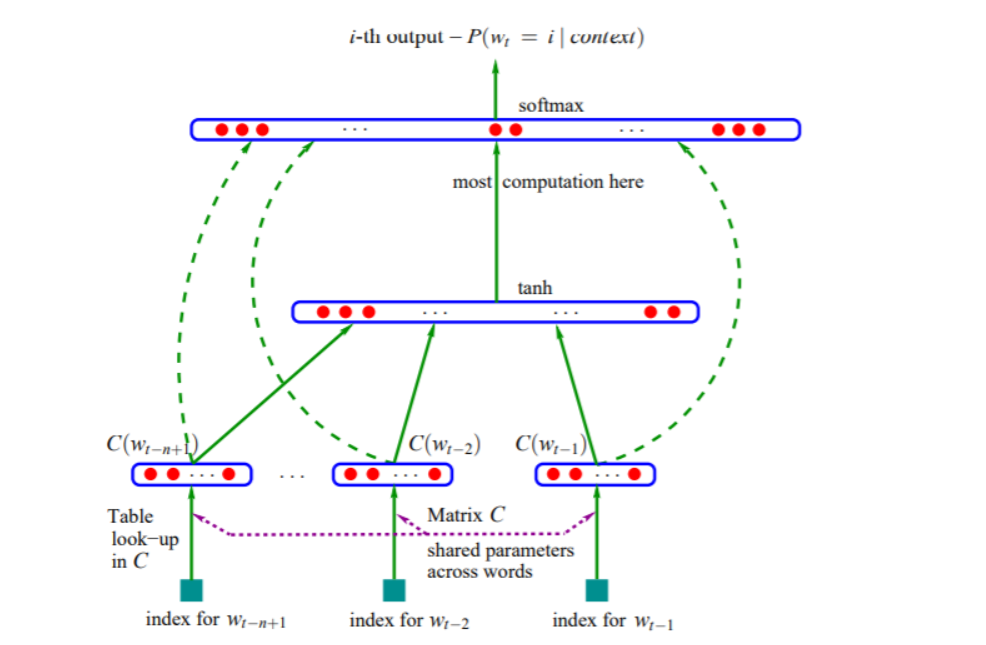
\includegraphics[width=\linewidth]{first_neural_lm}
	\captionof{figure}{Схема первой нейросетевой языковой модели}
\end{figure}

Следующий прорыв в языковом моделировании случился в 2013 году. Это связано с появлением Word2Vec --- универсальными векторными представлениями слов, разработанными Google. Векторные представления обучены на большом объеме данных, что позволяет хорошо отражать смысл слов. Это значит, что схожим по смыслу и значения словам будут соответствовать близкие по косиноснуму расстоянию вектора. Также исследования показали, что такие представления имеют некоторую линейную зависимость, которая выражается в подобных примерах: $king - man + woman \approx queen$.
Представления Word2Vec могут быть получены на больших объемах неразмеченных текстовых данных с помощью двух методов: Skip-gram и Continous Bag of Words (CBoW). Skip-gram основан на предсказании по данному слову его контекста, а CBoW наоборот --- пытается угадать слово по заданному контексту (Рис. 1.2). Также есть способы улучшить качество векторов и скорость сходимости, например, negative sampling, при котором кроме приближения схожих слов семплируются несколько случайных, и алгоритм пытается «отдалить» друг от друга слова, отличающиеся по смыслу.

\begin{figure}[ht]
	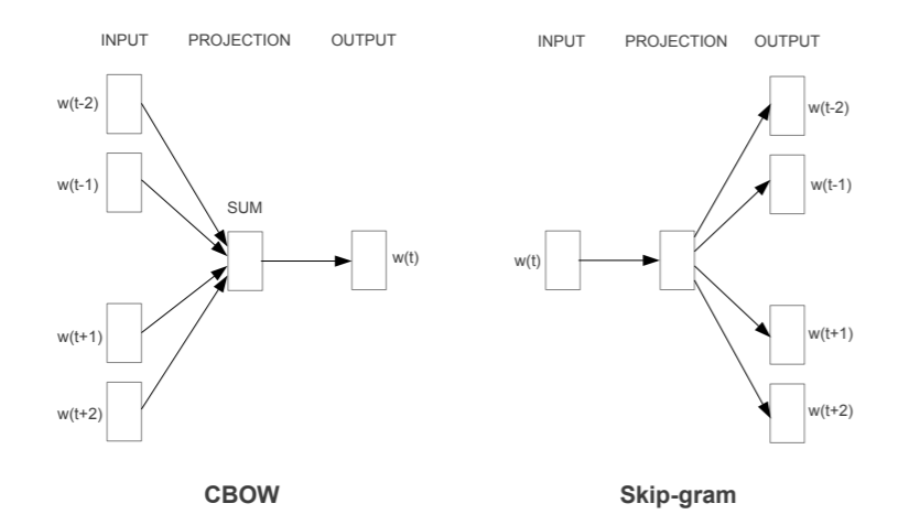
\includegraphics[width=\linewidth]{skip_gram_cbow}
	\captionof{figure}{Skip-gram и CBoW}
\end{figure}

Через год после успеха Word2Vec появился GloVe --- аналогичные векторные представления слов, которые показали себя лучше для ряда задач: поиск схожих слов и NER (Рис. 1.3). GloVe отличается исходными данными для обучения, а также основан на более сложном алгоритме.~\cite{twds-lm-history}

\begin{figure}[ht]
	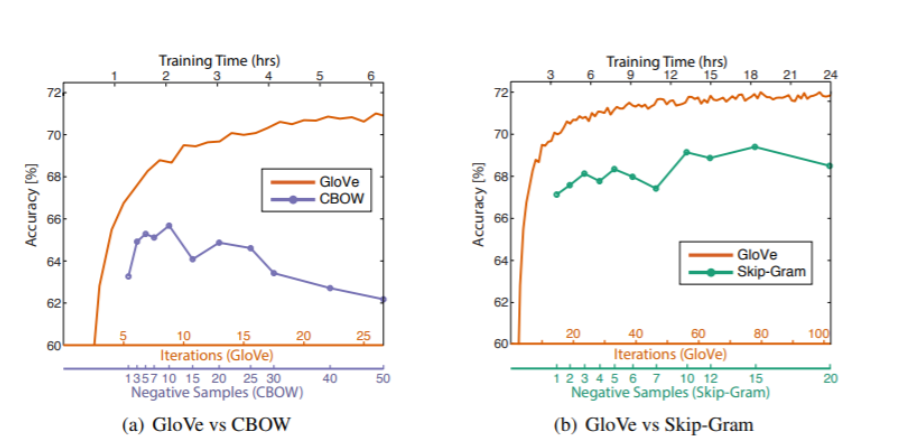
\includegraphics[width=\linewidth]{glove_vs_word2vec}
	\captionof{figure}{GloVe vs Word2Vec}
\end{figure}

Одновременно с GloVe в 2014 году были созданы сверточные нейронные сети ~\cite{kalchbrenner-etal-2014-convolutional}. Основной сферой применения сверточных сетей является компьютерное зрение, так как по своей природе они наиболее удачно подходят для обработки изображений, однако их можно применять и к текстовым данным. Наряду с рекуррентными сетями, сверточные сети были одним из основных направлений исследований в NLP.

Несмотря на то, что рекуррентные сети являются наиболее очевидным выбором для работы с последовательностями переменной длины, их обучение затруднялось особенностями архитектуры, а также такими феноменами, как затухающие и взрывающиеся градиенты, которые влиялии на вычислительную стабильность обратного распространения градиентов. Довольно большой вклад в решение данных проблем внес phd тезис~\cite{sutskever2013training}, в котором приводились результаты успешных экспериментов для различных задач, не только языкового моделирования, которые доказали возможность качественного обучения рекуррентных сетей.

Следующим шагом в развитии моделей для обработки последовательностей были Sequence to Sequence модели (seq2seq). В этой структуре нейронная сеть кодировщика обрабатывает предложение по одному токену и сжимает его в векторное представление; затем нейронная сеть декодера предсказывает выходные символы на основе состояния кодировщика, принимая в качестве входных данных на каждом шаге ранее предсказанный символ (Рис. 1.4)

\begin{figure}[ht]
	\centering
	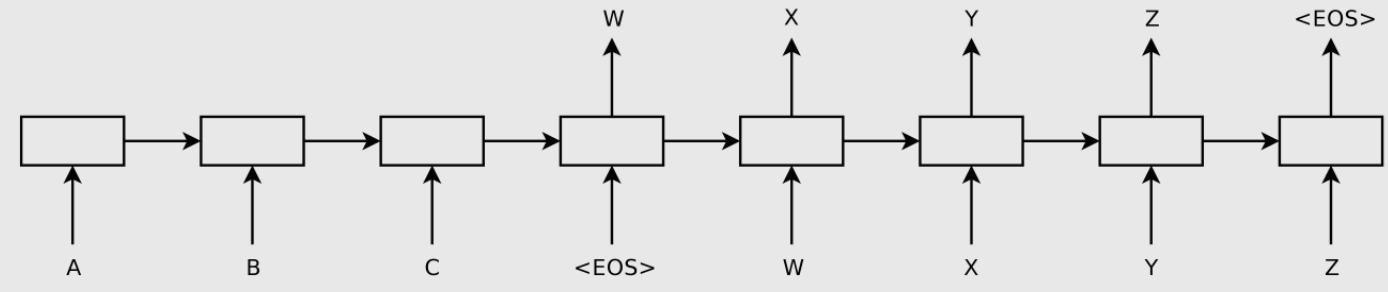
\includegraphics[width=\linewidth]{seq2seq2014}  
	\caption{ Схема seq2seq модели }
\end{figure}

Seq2seq благодаря своей гибкости в настоящее время является основным фреймворком для задач генерации естественного языка, при этом различные модели берут на себя роль кодировщика и декодера. Важно отметить, что модель декодера может быть обусловлена не только последовательностью, но и произвольными представлениями. Это позволяет, например, генерировать заголовок на основе изображения (Image Captioning)~\cite{image-captioning}. Здесь в качестве кодировщика применяется сверточная сеть, которая выдает сжатые представления изображений. Далее этот вектор идет на вход декодера, который выдает одно за другим слова заголовка (Рис 1.5).
\begin{figure}[ht]
	\centering
	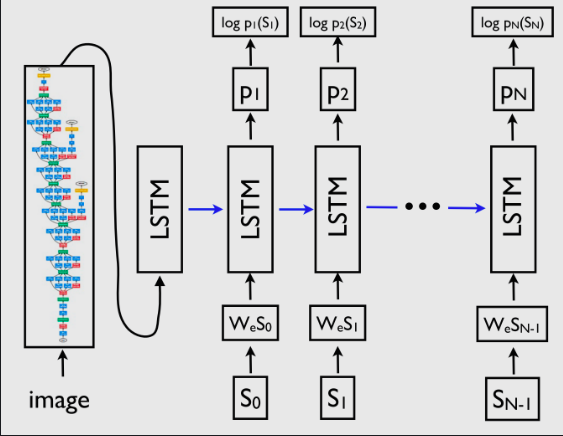
\includegraphics[width=\linewidth]{image_captioning}  
	\caption{ Архитектура seq2seq модели для генерации заголовков к изображениям }
\end{figure}

У модели seq2seq есть один значитеьный недостаток, который ограничивает качество моделей, --- вся входная информация сжимается в один вектор, который в дальнейшем используется в рекуррентной сети. 

\subsection{N-грамные модели}
\label{sub:domain:n_gram}


\subsubsection{Laplace Smoothing}

\subsubsection{Kneser-Nay smoothing}

\subsection{Нейросетевые модели}
\label{sub:domain:neural}



\subsubsection{Сверточные сети}

\subsubsection{Рекуррентные сети}

\subsubsection{Self-attention и трансформеры}

\subsection{Современные подходы к языковому моделированию}
\label{sub:domain:curr}

